
%% bare_conf.tex
%% V1.4b
%% 2015/08/26
%% by Michael Shell
%% See:
%% http://www.michaelshell.org/
%% for current contact information.
%%
%% This is a skeleton file demonstrating the use of IEEEtran.cls
%% (requires IEEEtran.cls version 1.8b or later) with an IEEE
%% conference paper.
%%
%% Support sites:
%% http://www.michaelshell.org/tex/ieeetran/
%% http://www.ctan.org/pkg/ieeetran
%% and
%% http://www.ieee.org/

%%*************************************************************************
%% Legal Notice:
%% This code is offered as-is without any warranty either expressed or
%% implied; without even the implied warranty of MERCHANTABILITY or
%% FITNESS FOR A PARTICULAR PURPOSE! 
%% User assumes all risk.
%% In no event shall the IEEE or any contributor to this code be liable for
%% any damages or losses, including, but not limited to, incidental,
%% consequential, or any other damages, resulting from the use or misuse
%% of any information contained here.
%%
%% All comments are the opinions of their respective authors and are not
%% necessarily endorsed by the IEEE.
%%
%% This work is distributed under the LaTeX Project Public License (LPPL)
%% ( http://www.latex-project.org/ ) version 1.3, and may be freely used,
%% distributed and modified. A copy of the LPPL, version 1.3, is included
%% in the base LaTeX documentation of all distributions of LaTeX released
%% 2003/12/01 or later.
%% Retain all contribution notices and credits.
%% ** Modified files should be clearly indicated as such, including  **
%% ** renaming them and changing author support contact information. **
%%*************************************************************************


% *** Authors should verify (and, if needed, correct) their LaTeX system  ***
% *** with the testflow diagnostic prior to trusting their LaTeX platform ***
% *** with production work. The IEEE's font choices and paper sizes can   ***
% *** trigger bugs that do not appear when using other class files.       ***                          ***
% The testflow support page is at:
% http://www.michaelshell.org/tex/testflow/



\documentclass[conference]{IEEEtran}
% Some Computer Society conferences also require the compsoc mode option,
% but others use the standard conference format.
%
% If IEEEtran.cls has not been installed into the LaTeX system files,
% manually specify the path to it like:
% \documentclass[conference]{../sty/IEEEtran}


\usepackage{cite}
\usepackage{amsmath,amssymb,amsfonts}
\usepackage{algorithmic}
\usepackage{graphicx}
\usepackage{textcomp}
\usepackage{xcolor}

\usepackage{pgfplots} % per a graficar amb LaTeX
\pgfplotsset{samples=2000} % número màxim de punts d'una corba que genera ell, canviar
\pgfplotsset{compat=1.16} % perquè si no el pgfplot dóna error
\usepackage{import} % per a les imatges d'Inkscape
\usepackage{xifthen} % per a les imatges d'Inkscape
\usepackage{pdfpages} % per a les imatges d'Inkscape
\usepackage{transparent} % per a les imatges d'Inkscape
\usepackage[RPvoltages]{circuitikz} % per tal que no salti warning
\usetikzlibrary{arrows, decorations.markings, arrows.meta} % per a dibuixar fletxes d'intensitat
\usepackage{gensymb}
\usepackage{steinmetz}


% Some very useful LaTeX packages include:
% (uncomment the ones you want to load)


% *** MISC UTILITY PACKAGES ***
%
%\usepackage{ifpdf}
% Heiko Oberdiek's ifpdf.sty is very useful if you need conditional
% compilation based on whether the output is pdf or dvi.
% usage:
% \ifpdf
%   % pdf code
% \else
%   % dvi code
% \fi
% The latest version of ifpdf.sty can be obtained from:
% http://www.ctan.org/pkg/ifpdf
% Also, note that IEEEtran.cls V1.7 and later provides a builtin
% \ifCLASSINFOpdf conditional that works the same way.
% When switching from latex to pdflatex and vice-versa, the compiler may
% have to be run twice to clear warning/error messages.






% *** CITATION PACKAGES ***
%
%\usepackage{cite}
% cite.sty was written by Donald Arseneau
% V1.6 and later of IEEEtran pre-defines the format of the cite.sty package
% \cite{} output to follow that of the IEEE. Loading the cite package will
% result in citation numbers being automatically sorted and properly
% "compressed/ranged". e.g., [1], [9], [2], [7], [5], [6] without using
% cite.sty will become [1], [2], [5]--[7], [9] using cite.sty. cite.sty's
% \cite will automatically add leading space, if needed. Use cite.sty's
% noadjust option (cite.sty V3.8 and later) if you want to turn this off
% such as if a citation ever needs to be enclosed in parenthesis.
% cite.sty is already installed on most LaTeX systems. Be sure and use
% version 5.0 (2009-03-20) and later if using hyperref.sty.
% The latest version can be obtained at:
% http://www.ctan.org/pkg/cite
% The documentation is contained in the cite.sty file itself.






% *** GRAPHICS RELATED PACKAGES ***
%
\ifCLASSINFOpdf
  % \usepackage[pdftex]{graphicx}
  % declare the path(s) where your graphic files are
  % \graphicspath{{../pdf/}{../jpeg/}}
  % and their extensions so you won't have to specify these with
  % every instance of \includegraphics
  % \DeclareGraphicsExtensions{.pdf,.jpeg,.png}
\else
  % or other class option (dvipsone, dvipdf, if not using dvips). graphicx
  % will default to the driver specified in the system graphics.cfg if no
  % driver is specified.
  % \usepackage[dvips]{graphicx}
  % declare the path(s) where your graphic files are
  % \graphicspath{{../eps/}}
  % and their extensions so you won't have to specify these with
  % every instance of \includegraphics
  % \DeclareGraphicsExtensions{.eps}
\fi
% graphicx was written by David Carlisle and Sebastian Rahtz. It is
% required if you want graphics, photos, etc. graphicx.sty is already
% installed on most LaTeX systems. The latest version and documentation
% can be obtained at: 
% http://www.ctan.org/pkg/graphicx
% Another good source of documentation is "Using Imported Graphics in
% LaTeX2e" by Keith Reckdahl which can be found at:
% http://www.ctan.org/pkg/epslatex
%
% latex, and pdflatex in dvi mode, support graphics in encapsulated
% postscript (.eps) format. pdflatex in pdf mode supports graphics
% in .pdf, .jpeg, .png and .mps (metapost) formats. Users should ensure
% that all non-photo figures use a vector format (.eps, .pdf, .mps) and
% not a bitmapped formats (.jpeg, .png). The IEEE frowns on bitmapped formats
% which can result in "jaggedy"/blurry rendering of lines and letters as
% well as large increases in file sizes.
%
% You can find documentation about the pdfTeX application at:
% http://www.tug.org/applications/pdftex





% *** MATH PACKAGES ***
%
%\usepackage{amsmath}
% A popular package from the American Mathematical Society that provides
% many useful and powerful commands for dealing with mathematics.
%
% Note that the amsmath package sets \interdisplaylinepenalty to 10000
% thus preventing page breaks from occurring within multiline equations. Use:
%\interdisplaylinepenalty=2500
% after loading amsmath to restore such page breaks as IEEEtran.cls normally
% does. amsmath.sty is already installed on most LaTeX systems. The latest
% version and documentation can be obtained at:
% http://www.ctan.org/pkg/amsmath





% *** SPECIALIZED LIST PACKAGES ***
%
%\usepackage{algorithmic}
% algorithmic.sty was written by Peter Williams and Rogerio Brito.
% This package provides an algorithmic environment fo describing algorithms.
% You can use the algorithmic environment in-text or within a figure
% environment to provide for a floating algorithm. Do NOT use the algorithm
% floating environment provided by algorithm.sty (by the same authors) or
% algorithm2e.sty (by Christophe Fiorio) as the IEEE does not use dedicated
% algorithm float types and packages that provide these will not provide
% correct IEEE style captions. The latest version and documentation of
% algorithmic.sty can be obtained at:
% http://www.ctan.org/pkg/algorithms
% Also of interest may be the (relatively newer and more customizable)
% algorithmicx.sty package by Szasz Janos:
% http://www.ctan.org/pkg/algorithmicx




% *** ALIGNMENT PACKAGES ***
%
%\usepackage{array}
% Frank Mittelbach's and David Carlisle's array.sty patches and improves
% the standard LaTeX2e array and tabular environments to provide better
% appearance and additional user controls. As the default LaTeX2e table
% generation code is lacking to the point of almost being broken with
% respect to the quality of the end results, all users are strongly
% advised to use an enhanced (at the very least that provided by array.sty)
% set of table tools. array.sty is already installed on most systems. The
% latest version and documentation can be obtained at:
% http://www.ctan.org/pkg/array


% IEEEtran contains the IEEEeqnarray family of commands that can be used to
% generate multiline equations as well as matrices, tables, etc., of high
% quality.




% *** SUBFIGURE PACKAGES ***
%\ifCLASSOPTIONcompsoc
%  \usepackage[caption=false,font=normalsize,labelfont=sf,textfont=sf]{subfig}
%\else
%  \usepackage[caption=false,font=footnotesize]{subfig}
%\fi
% subfig.sty, written by Steven Douglas Cochran, is the modern replacement
% for subfigure.sty, the latter of which is no longer maintained and is
% incompatible with some LaTeX packages including fixltx2e. However,
% subfig.sty requires and automatically loads Axel Sommerfeldt's caption.sty
% which will override IEEEtran.cls' handling of captions and this will result
% in non-IEEE style figure/table captions. To prevent this problem, be sure
% and invoke subfig.sty's "caption=false" package option (available since
% subfig.sty version 1.3, 2005/06/28) as this is will preserve IEEEtran.cls
% handling of captions.
% Note that the Computer Society format requires a larger sans serif font
% than the serif footnote size font used in traditional IEEE formatting
% and thus the need to invoke different subfig.sty package options depending
% on whether compsoc mode has been enabled.
%
% The latest version and documentation of subfig.sty can be obtained at:
% http://www.ctan.org/pkg/subfig




% *** FLOAT PACKAGES ***
%
%\usepackage{fixltx2e}
% fixltx2e, the successor to the earlier fix2col.sty, was written by
% Frank Mittelbach and David Carlisle. This package corrects a few problems
% in the LaTeX2e kernel, the most notable of which is that in current
% LaTeX2e releases, the ordering of single and double column floats is not
% guaranteed to be preserved. Thus, an unpatched LaTeX2e can allow a
% single column figure to be placed prior to an earlier double column
% figure.
% Be aware that LaTeX2e kernels dated 2015 and later have fixltx2e.sty's
% corrections already built into the system in which case a warning will
% be issued if an attempt is made to load fixltx2e.sty as it is no longer
% needed.
% The latest version and documentation can be found at:
% http://www.ctan.org/pkg/fixltx2e


%\usepackage{stfloats}
% stfloats.sty was written by Sigitas Tolusis. This package gives LaTeX2e
% the ability to do double column floats at the bottom of the page as well
% as the top. (e.g., "\begin{figure*}[!b]" is not normally possible in
% LaTeX2e). It also provides a command:
%\fnbelowfloat
% to enable the placement of footnotes below bottom floats (the standard
% LaTeX2e kernel puts them above bottom floats). This is an invasive package
% which rewrites many portions of the LaTeX2e float routines. It may not work
% with other packages that modify the LaTeX2e float routines. The latest
% version and documentation can be obtained at:
% http://www.ctan.org/pkg/stfloats
% Do not use the stfloats baselinefloat ability as the IEEE does not allow
% \baselineskip to stretch. Authors submitting work to the IEEE should note
% that the IEEE rarely uses double column equations and that authors should try
% to avoid such use. Do not be tempted to use the cuted.sty or midfloat.sty
% packages (also by Sigitas Tolusis) as the IEEE does not format its papers in
% such ways.
% Do not attempt to use stfloats with fixltx2e as they are incompatible.
% Instead, use Morten Hogholm'a dblfloatfix which combines the features
% of both fixltx2e and stfloats:
%
% \usepackage{dblfloatfix}
% The latest version can be found at:
% http://www.ctan.org/pkg/dblfloatfix




% *** PDF, URL AND HYPERLINK PACKAGES ***
%
%\usepackage{url}
% url.sty was written by Donald Arseneau. It provides better support for
% handling and breaking URLs. url.sty is already installed on most LaTeX
% systems. The latest version and documentation can be obtained at:
% http://www.ctan.org/pkg/url
% Basically, \url{my_url_here}.




% *** Do not adjust lengths that control margins, column widths, etc. ***
% *** Do not use packages that alter fonts (such as pslatex).         ***
% There should be no need to do such things with IEEEtran.cls V1.6 and later.
% (Unless specifically asked to do so by the journal or conference you plan
% to submit to, of course. )


% correct bad hyphenation here
\hyphenation{op-tical net-works semi-conduc-tor}


\begin{document}
%
% paper title
% Titles are generally capitalized except for words such as a, an, and, as,
% at, but, by, for, in, nor, of, on, or, the, to and up, which are usually
% not capitalized unless they are the first or last word of the title.
% Linebreaks \\ can be used within to get better formatting as desired.
% Do not put math or special symbols in the title.
\title{AC/DC Power Flow modelled with the Flexible General Branch Model and solved with the Holomorphic Embedding Method}


% author names and affiliations
% use a multiple column layout for up to three different
% affiliations
\author{\IEEEauthorblockN{Josep Fanals Batllori}
\IEEEauthorblockA{u1946589@campus.udg.edu}}


% conference papers do not typically use \thanks and this command
% is locked out in conference mode. If really needed, such as for
% the acknowledgment of grants, issue a \IEEEoverridecommandlockouts
% after \documentclass

% for over three affiliations, or if they all won't fit within the width
% of the page, use this alternative format:
% 
%\author{\IEEEauthorblockN{Michael Shell\IEEEauthorrefmark{1},
%Homer Simpson\IEEEauthorrefmark{2},
%James Kirk\IEEEauthorrefmark{3}, 
%Montgomery Scott\IEEEauthorrefmark{3} and
%Eldon Tyrell\IEEEauthorrefmark{4}}
%\IEEEauthorblockA{\IEEEauthorrefmark{1}School of Electrical and Computer Engineering\\
%Georgia Institute of Technology,
%Atlanta, Georgia 30332--0250\\ Email: see http://www.michaelshell.org/contact.html}
%\IEEEauthorblockA{\IEEEauthorrefmark{2}Twentieth Century Fox, Springfield, USA\\
%Email: homer@thesimpsons.com}
%\IEEEauthorblockA{\IEEEauthorrefmark{3}Starfleet Academy, San Francisco, California 96678-2391\\
%Telephone: (800) 555--1212, Fax: (888) 555--1212}
%\IEEEauthorblockA{\IEEEauthorrefmark{4}Tyrell Inc., 123 Replicant Street, Los Angeles, California 90210--4321}}




% use for special paper notices
%\IEEEspecialpapernotice{(Invited Paper)}




% make the title area
\maketitle

% As a general rule, do not put math, special symbols or citations
% in the abstract
\begin{abstract}
This paper covers the fundamental formulation regarding the combination of a Flexible General Branch Model (FGBM) with the holomorphic embedding method. The FGBM defines the links between buses with a common and complete model which not only works for AC networks but is also useful for DC grids and the conversion types of currents. It has proven to be a successful choice along with the Newton-Raphson method.

The holomorphic embedding method is a non-iterative totally reliable algorithm with a potential edge in comparison to the traditional iterative algorithms. Up to this point in time, it has been used for AC grids and DC components, but no work in the literature covers the AC/DC power flow. This paper establishes the bases for exactly that and shows its applicability in a simple two-bus system.

\end{abstract}
\begin{IEEEkeywords}
power flow, holomorphic embedding, AC/DC, convergence, rectifier, inverter
\end{IEEEkeywords}  

% no keywords




% For peer review papers, you can put extra information on the cover
% page as needed:
% \ifCLASSOPTIONpeerreview
% \begin{center} \bfseries EDICS Category: 3-BBND \end{center}
% \fi
%
% For peerreview papers, this IEEEtran command inserts a page break and
% creates the second title. It will be ignored for other modes.
\IEEEpeerreviewmaketitle

\section{Introduction}\label{secIntro}
The current European power systems are about to undertake massive changes due to EU's policies, which are concerned with the security of energy supply, the competitiveness of electricity markets and the sustainability aspect. Supergrids are being created in order to accommodate this incoming evolution. They use Voltage Source Converters (VSC) and HVDC grids, apart from the current AC system. HVDC offers great flexibility of operation as well as the possibility of multiterminal configurations \cite{Bompard}.

Due to that, the modern supergrid will include a considerable percentage of renewable energy sources, like solar power and wind power choices. Specially in Europe, the concept of offshore wind power has been studied in depth \cite{Gomis}. 

Therefore, it is critical to work with a flexible model of the grid while solving the power flow with reliable tools. The FGBM is detailed in \cite{alvarez}. The authors depict the proposed model and employ it to solve successfully a multiterminal DC grid that connects with AC systems. However, the usage of the NR method could yield infeasible results. On the other hand, the holomorphic embedding method obtains the feasible solution when it exists. It also grants extra information with tools like Sigma and Thévenin approximants.

The holomorphic embedding method is a novel technique that first appeared in \cite{Trias2012} as a revolutionary algorithm based on complex analysis, algebraic curves and approximation theory. It has been used for AC power flow analysis as well as for DC components such as diodes or solar panels. Despite that, the state of art does not cover the conversion between AC/DC grids. It is possible that the tools in which the holomorphic embedding method is based could be extended to the supergrid of the future accompanied by VSC, HVDC, FACTS and overall an increasing number of power electronics elements.

This paper is structured as follows: Section \ref{secEquacions} presents the equations involved in a simple two-bus system; Section \ref{secEmbed} embeds these equations and presents the algorithm that has to be followed; Section \ref{secResults} shows the results obtained and discusses them; finally, Section \ref{secConcl} concludes the paper.


\section{Formulation}\label{secEquacions}
A simple system such as the one in Figure \ref{fig:sistema} is selected in order to introduce the adaptation of the holomorphic embedding method to solve the AC/DC power flow.
\begin{figure}[!htb]
  \begin{center}
  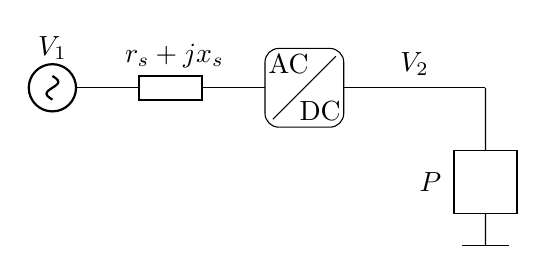
\begin{tikzpicture}[scale = 1, transform shape]
    \draw (-2, 0) to [/tikz/circuitikz/bipoles/length=1.0cm, sV] (-1.4, 0);
    \ctikzset{resistor = european}
    \draw (-1.4, 0) to [/tikz/circuitikz/bipoles/length=1.0cm, resistor] (1, 0);
    % \draw (0.6, 0) to [/tikz/circuitikz/bipoles/length=1.0cm, resistor] (4, 0);
    % \draw [line width=0.75] (4.25, 0) circle (0.25);
    % \draw [line width=0.75] (4.5, 0) circle (0.25);
    % \draw (4.75, 0) to [short] (5.2, 0);
    % \draw (5.2, 0) to [short, i_=$I_s\phase{\phi}$] (6.0, 0);
    % \draw (6.0, 0) to [short] (6.15, 0);
    % \draw (6.15+0.4, -0.3) to [/tikz/circuitikz/bipoles/length=0.8cm, empty diode] (6.15+0.4, 0.3);
    % \draw [line width=0.75] (6.15, -0.4) -- (6.15, 0.4);
    % \draw [line width=0.75] (6.95, -0.4) -- (6.95, 0.4);
    % \draw [line width=0.75] (6.15, -0.4) -- (6.95, -0.4);
    % \draw [line width=0.75] (6.15, 0.4) -- (6.95, 0.4);
    % \draw (6.55, 0.4) -- (6.55, 1.0);
    % \draw (6.55, -0.4) -- (6.55, -1.0);
    % \draw (6.55, 1.0) to [short, i=$I_{DC}$] (7.7, 1.0);
    % \draw (6.55, -1.0) -- (7.7, -1.0);
    % \ctikzset{resistor = american}
    % \draw (7.7, -1.0) to [/tikz/circuitikz/bipoles/length=0.8cm, resistor, l=$R$,v_=$V_{DC}$] (7.7, 1.0);
    % \draw [line width=2] (1.2, -0.4) -- (1.2, 0.4);
    % \draw [line width=2] (3.675, -0.4) -- (3.675, 0.4);
    % \draw [line width=2] (5.1, -0.4) -- (5.1, 0.4);
    % \draw (4.67, 0.51) node[anchor=south west] {$E\phase{\psi}$};
    % \draw (3.25, 0.45) node[anchor=south west] {$V\phase{\theta}$};
    % \draw (0.78, 0.45) node[anchor=south west] {$U\phase{0}$};
    % \draw (1.95, 0.1) node[anchor=south west] {$\vec{Z_L}$};
    % \draw (2.9, 0) to [short, i_=$I_p\phase{\gamma}$] (3.4, 0);
    % \draw (4.15, -0.60) node[anchor=south west] {$a$};

    \draw[rounded corners=5pt] (1,-0.5) rectangle (2.0,0.5);
  \draw (1.1,-0.4) -- (1.9,0.4);
  \node at (1.3,0.3) {AC};
  \node at (1.7,-0.3) {DC};
  \draw (3.8, 0) to [short] (3.8, -0.8);
  \draw (3.4, -1.6) rectangle (4.2, -0.8);
  \draw (3.8, -1.6) to [short] (3.8, -2);
  \draw (3.5, -2) to [short] (4.1, -2);
  \node at (-1.7,0.5) {$V_1$};
  \node at (2.9,0.3) {$V_2$};
  \draw (2.0, 0) to [short] (3.8, 0);
  \node at (3.1, -1.2) {$P$};
  \node at (-0.15, 0.4) {$r_s + jx_s$};


  \end{tikzpicture}
  \caption{Simplified system with the AC/DC converter}
  \label{fig:sistema}
  \end{center}
  \end{figure}

The slack bus is represented by $V_1$, which is known. The reference is established in this exact same bus. The FGBM allows the reference to only be set in a single bus and not having to decouple between AC and DC systems. The most complete FGBM model is employed for the VSC, which links an AC bus with a DC bus, or rather, a DC bus with an AC bus, since the DC bus is indexed by $f$ (from) and the AC one with $t$ (to).

Once the converter is surpassed, the connections between DC buses would obey the traditional model that integrates a single resistance, i.e. $x_s=0$ and $b_c=0$. There is no further complication on this side of the system. In this case, only a constant power load has been placed. The hardest part to model is found in the conversion from AC to DC. According to \cite{alvarez}, in each DC network there has to be a single type II converter (it could also be a type III). The remaining converters follow the type I constraints. Due to that, in this example the only converter will be type II, and more in depth, the control mode number 5 is applied.

Therefore, the DC voltage will be known (not its phase, only its absolute value) and also the AC bus. Indeed, the slack bus is not treated as an unknown. Usually, three variables emerge from every converter: $\theta_{sh}$, $m_a$ and $B_{eq}$. Fortunately, $\theta_{sh}=0$ and $m_a=1$ due to the fact that the only controlled variable is $V_2$, or rather, $v_{dc}$.

Quite straightforwardly, the first equation to derive connects the current $I_f$ (the one leaving the DC bus in direction to the slack bus) with the whole system:
\begin{equation}
  \begin{split}
    I_f = y_s(V_2 - V_1) + j \frac{b_c}{2}V_2 + jB_{eq}V_2 + G|I_f|^2V_2,
  \end{split}
  \label{eq:int1}
\end{equation}
where several changes of variables where introduced. $G = \frac{G_0}{I^2_{f,nom}}$ and $y_s=\frac{1}{r_s+jx_s}$. The equation results from the admittance matrix taking into account the aforementioned values of the converter.

The next equation to take into account has to do with the constant complex power load located in the DC side of the system. The beauty of this methodology is found in that all voltages and currents are complex variables, yet reactive power disappears because the DC phases match (or are rotated $\pi$ radians). Thus
\begin{equation}
  P + 0j = V_2 I^*_f.
  \label{eq:p1}
\end{equation}
Finally there is an equation left to consider. Because the converter operates following the II control model, $v_{dc}$ is part of the data. It has to be treated similarly to a PV bus of a classical AC grid. The absolute value is known but its phase not yet. 
\begin{equation}
  W = |V_2|^2,
  \label{eq:vabs1}
\end{equation}
where $W$ is a given value. 

At this stage of the formulation, the system of equations constituted by \eqref{eq:int1}, \eqref{eq:p1} and \eqref{eq:vabs1} appears to be nonlinear. Consequently, an iterative method like the well-known Newton-Raphson could be employed. Nevertheless, this paper will present a formulation based on the holomorphic embedding method. No paper covers the AC/DC conversion with that last approach, and on the other hand, the FGBM allows the usage of Sigma approximants to diagnose the state of the system. 


\section{Embedding}\label{secEmbed}
The holomorphic embedding method is based on embedding the equations involved. Embedding means that the problem is submerged inside a bigger problem. After a reference state is obtained, the solution can be extended up to the operative state. The choice of embedding is not unique. Despite that, the canonical embedding is a tested alternative that works adequately. It states that $V_i[0]=1 \hspace{5pt} \forall i$ and $I_i[0]=0 \hspace{5pt} \forall i$.

Therefore, \eqref{eq:int1} develops into
\begin{equation}
  \begin{split}
  I_f(s) &= y_sV_2(s) - y_sV_1(s) + s j \frac{b_c}{2}V_2(s) + s j B_{eq}(s) V_2(s) \\
  &+ s G |I_f(s)|^2 V_2(s).
  \end{split}
  \label{eq:int2}
\end{equation}
Note that only $I_f(s)$ and the terms including $y_s$ do not multiply directly by $s$. This way they are the responsible for conforming the reference state. $V_1(s)$ responds to the typical embedding for slack buses
\begin{equation}
  V_1(s) = 1 + s(V_1 - 1),
  \label{eq:slack}
\end{equation}
where $V_1$ is the known voltage with the reference angle set at 0. It is convenient to expand \eqref{eq:int2} further to avoid $|I_f(s)|^2$
\begin{equation}
  \begin{split}
    I_f(s) &= y_sV_2(s) - y_sV_1(s) + s j \frac{b_c}{2}V_2(s) + s j B_{eq}(s) V_2(s) \\
    &+ s G I^{(re)}_f(s)I^{(re)}_f(s)I^{(im)}_f(s)I^{(im)}_f(s) V_2(s),
    \end{split}
  \label{eq:int3}
\end{equation}
where $I^{(re)}_f(s)$ and $I^{(im)}_f(s)$ are the real and imaginary part of $I_f(s)$ respectively.

When it comes to \eqref{eq:p1}, the variables should also be fragmented into real and imaginary part. 
\begin{equation}
  sP+0j=(V^{(re)}_2(s) + jV^{(im)}_2(s))(I^{(re)}_f(s) - jI^{(im)}_f(s)).
  \label{eq:p2}
\end{equation}
This way the resulting system of equations will not be concerned with obtaining the absolute value and the phases like the Newton-Raphson would. Instead, the real and imaginary parts will be computed akin to the traditional holomorphic embedding method. 

Lastly, \eqref{eq:vabs1} adopts the form
\begin{equation}
  1 + s(W - 1) = V^{(re)}_2(s)V^{(re)}_2(s) + V^{(im)}_2(s)V^{(im)}_2(s).
  \label{eq:vabs2}
\end{equation}
From \eqref{eq:int3}, \eqref{eq:p2} and \eqref{eq:vabs2} it can be checked that all these equations are compatible with the desired reference state. Moreover, the $c$ term that builds $B_{eq}(s)$ will be obtained at the same time the $c+1$ coefficient of the other variables is obtained. In other words, its calculation will always be a step behind.

A system of 5 equations is derived from \eqref{eq:int3}, \eqref{eq:p2} and \eqref{eq:vabs2}, since the first two are complex a generalized system at depth $c$ becomes
\begin{equation}
  \begin{pmatrix}
    1 & 0 & -g & b & 0\\
    0 & 1 & -b & -g & -1\\
    1 & 0 & 0 & 0 & 0\\
    0 & 1 & 0 & 0 & 0\\
    0 & 0 & 2 & 0 & 0\\
  \end{pmatrix}
  \begin{pmatrix}
    I_f^{(re)}[c]\\
    I_f^{(im)}[c]\\
    V^{(re)}_2[c]\\
    V^{(im)}_2[c]\\
    B_{eq}[c-1]\\
  \end{pmatrix}
  =RHS[c],
  \label{eq:matriu}
\end{equation}
where it has already been considered that $V_2[0]=1$. It only remains to construct the $RHS$ vector. The terms that intervene in \eqref{eq:int3} and build $RHS$ at the first stage turn out to be
\begin{equation}
  \begin{split}
  A &= -g(V_1 - 1) + GV_2[0]\left(I^{(re)}_f[0]^2 + I^{(im)}_f[0]^2\right)\\ 
  &- b(V_1 - 1) + j\frac{b_c}{2}V_2[0],
  \end{split}
  \label{eq:A}
\end{equation}
where $g+jb=y_s$. From here
\begin{equation}
  RHS[1]=\begin{pmatrix}
    \Re[A]\\
    \Im[A]\\
    P\\
    0\\
    W-1\\
  \end{pmatrix}.
  \label{eq:rhs1}
\end{equation}
As a result of that, in order to obtain the first set of coefficients the matrix of \eqref{eq:matriu} has to be inverted (or factorized). In contrast to the Newton-Raphson scheme, here the matrix remains the same, independent of the order. From a computational time standpoint, although the holomorphic embedding method usually needs between 20 and 40 coefficients, each of its step is essentially faster than a Newton-Raphson iteration.  

For a generalized order $c\geq 2$ the $RHS$ expressions gain in complexity. For \eqref{eq:int3}
\begin{equation}
  \begin{split}
  A &= G\sum_{k=0}^{c-1}V_2[k]\sum_{j=0}^{c-1-k}I^{(re)}_f[j]I^{(re)}_f[c-1-k-j]\\
  & +G\sum_{k=0}^{c-1}V_2[k]\sum_{j=0}^{c-1-k}I^{(im)}_f[j]I^{(im)}_f[c-1-k-j]\\
  &+j(\frac{b_c}{2}V_2[c-1] + \sum_{k=1}^{c-1}V_2[k]B_{eq}[c-1-k]),
  \end{split}
  \label{eq:A2}
\end{equation}
where there are some double convolutions which are not worrying in the sense that the algorithm can still converge to the sought solution.

Then, the real part of \eqref{eq:p2} is converted into
\begin{equation}
    B=-\sum_{k=1}^{c-1}V^{(re)}_2[k]I^{(re)}_f[c-k]-\sum_{k=1}^{c-1}V^{(im)}_2[k]I^{(im)}_f[c-k],
  \label{eq:B}
\end{equation}
while the imaginary becomes
\begin{equation}
  C=-\sum_{k=1}^{c-1}V^{(im)}_2[k]I^{(re)}_f[c-k]-\sum_{k=1}^{c-1}V^{(re)}_2[k]I^{(im)}_f[c-k].
\label{eq:C}
\end{equation}
Finally, there is only one expression left to consider. From \eqref{eq:vabs2} the expansion of coefficients yields
\begin{equation}
  D = -\sum_{k=1}^{c-1}V^{(re)}_2[k]V^{(re)}_2[c-k]-\sum_{k=1}^{c-1}V^{(im)}_2[k]V^{(im)}_2[c-k].
  \label{eq:D}
\end{equation}
All this allows the construction of the definitive $RHS$ vector
\begin{equation}
  RHS[c]=\begin{pmatrix}
    \Re[A]\\
    \Im[A]\\
    B\\
    C\\
    D\\
  \end{pmatrix}.
  \label{eq:rhsc}
\end{equation}
Thus, the algorithm has been fully built for any given order. Of course it would change depending on the dimensions of the system as well as the variables to control, but its core remains. From \eqref{eq:matriu} it can be seen that the dependence of $g$ and $b$ with the voltages is similar to the one encountered with AC systems, despite having changed the signs here.

\section{Results}\label{secResults}
To show that the holomorphic embedding is compatible with the FGBM some basic results are offered. The first and most convenient test to implement has to do with the errors and how the evolve according to the chosen depth. This alone is often enough to get a glimpse of the convergence properties of the series. An embedding that leads to convergent series is more appropriate that another that does not. However, both can generate a final correct solution. 

Table \ref{tab:1} captures the initial dataset of the problem expressed in per unit values.

\begin{table}[!ht]
  \renewcommand{\arraystretch}{1.0}
  \caption{Data of the simple AC/DC system}
  \label{tab:1}
  \centering
  \begin{tabular}{cc}
  \hline
  Magnitude & Value\\
  \hline
  $P$ & -0.2\\
  $V_1$ & 1.05\\
  $W$ & 0.95\\
  $g$ & 5\\
  $b$ & -10\\
  $G$ & 10\\
  $b_c$ & 100\\
  \hline
  \end{tabular}
  \end{table}

A negative $P$ value symbolizes active power demand. It has to be noted that all these numbers are made up and could be not totally congruent with the current real-life systems and converters.

Figure \ref{fig:0} plots the maximum error as a function of the number of coefficients used, both with Padé approximants and directly summing the terms. In this state the convergence properties are so favorable that Padé approximants do not provide any substantial advantage. From 25 coefficients onwards the error plateaus. Double-precision floating-point format was employed. 

\begin{figure}[!ht]\footnotesize
  \centering
  \begin{tikzpicture}
      \begin{axis}[
          /pgf/number format/.cd, ylabel={$\log|$Error$|$},xlabel={Number of coefficients},domain={-0.25:0.25},width=7cm,height=6.5cm,legend style={at={(1,1.0)},anchor=north east}, scatter/classes={%
        b={mark=x,mark size=1.5pt,draw=black},c={mark=o,mark size=1.5pt,draw=black}}]]
      \addplot[scatter, scatter src=explicit symbolic]%
          table[x = x, y = y, meta = label, col sep=semicolon] {Resultats/pade_basic.csv};
        \addplot[scatter, scatter src=explicit symbolic]%
        table[x = x, y = y, meta = label, col sep=semicolon] {Resultats/suma_basic.csv};
          \legend{, Padé, Sum}
      \end{axis}
      \end{tikzpicture}
  \caption{Maximum error depending on the depth}
  \label{fig:0}
  \end{figure}

  It is worth-telling that other models for the AC/DC conversion could also be used. however, the traditional ones as presented in \cite{Tylavsky}-\cite{Yang} when combined with the holomorphic embedding do not yield convergent results. In addition to that, it is hard to find a suitable embedding. Hence the relevance of the FGBM.

  Another representative result is the maximum power the DC load can consume so that the power flow is still feasible. As expected, the error should increase. Figure \ref{fig:1} plots the maximum error as a function of $P$ with a depth of 30 terms.

  \begin{figure}[!ht]\footnotesize
    \centering
    \begin{tikzpicture}
        \begin{axis}[
            /pgf/number format/.cd, ylabel={$\log|$Error$|$},xlabel={$|P|$},domain={-0.25:0.25},width=7cm,height=6.5cm,legend style={at={(0.00,1.0)},anchor=north west}, scatter/classes={%
          b={mark=x,mark size=1.5pt,draw=black},c={mark=o,mark size=1.5pt,draw=black}}]]
        \addplot[scatter, scatter src=explicit symbolic]%
            table[x = x, y = y, meta = label, col sep=semicolon] {Resultats/pade_evol.csv};
          \addplot[scatter, scatter src=explicit symbolic]%
          table[x = x, y = y, meta = label, col sep=semicolon] {Resultats/suma_evol.csv};
            \legend{, Sum, Padé}
        \end{axis}
        \end{tikzpicture}
    \caption{Maximum error depending on the active power load}
    \label{fig:1}
    \end{figure}

From what can be observed, for $|P|<0.3$ the error obtained with Padé or with the sum remains practically the same. Padé approximants become handy once $|P|$ increases. Despite following the same trend, its maximum error stays about 2 orders of magnitude below the one with the summation of coefficients.

It is also valuable to evaluate the variation of $B_{eq}$ depending on variations of $P$. Table \ref{tab:2} displays its value according to the selected $|P|$. The closer to 0 $|P|$ is, the smaller $B_{eq}$ gets. All in all, there is a weak link between these two variables.

\begin{table}[!ht]
  \renewcommand{\arraystretch}{1.0}
  \caption{$B_{eq}$ values as a function of $P$}
  \label{tab:2}
  \centering
  \begin{tabular}{cc}
  \hline
  $P$ & $B_{eq}$\\
  \hline
  0.6 & -48.86\\
  0.4 & -50.29\\
  0.2 & -50.86\\
  -0.2 & -50.65\\
  -0.4 & -49.73\\
  -0.6 & -47.50\\
  \hline
  \end{tabular}
  \end{table}

\section{Conclusion}\label{secConcl}
A functional combination of the holomorphic embedding method with the AC/DC power flow has been achieved for a simple test case where the series involved converged at a fast pace. The FGBM turns out to be an innovative adequate model which facilitates the combination of the AC power flow with the DC power flow with no need to decouple systems. 

This paper lands the foundation of the development of a full algorithm based on the holomorphic embedding able to solve realistic AC/DC systems. That would benefit from the resources that the holomorphic embedding offers: Thévenin approximants to plot accurate PV curves, Sigma approximants to diagnose the system and the Padé-Weierstrass to improve the solution when needed. The robustness of the holomorphic embedding is arguably greater than iterative methods, making it a possible ground-breaking tool to be applied in the AC/DC power flow.



% conference papers do not normally have an appendix


% use section* for acknowledgment
% \section*{Acknowledgment}
% The authors would like to thank...





% trigger a \newpage just before the given reference
% number - used to balance the columns on the last page
% adjust value as needed - may need to be readjusted if
% the document is modified later
%\IEEEtriggeratref{8}
% The "triggered" command can be changed if desired:
%\IEEEtriggercmd{\enlargethispage{-5in}}

% references section

% can use a bibliography generated by BibTeX as a .bbl file
% BibTeX documentation can be easily obtained at:
% http://mirror.ctan.org/biblio/bibtex/contrib/doc/
% The IEEEtran BibTeX style support page is at:
% http://www.michaelshell.org/tex/ieeetran/bibtex/
%\bibliographystyle{IEEEtran}
% argument is your BibTeX string definitions and bibliography database(s)
%\bibliography{IEEEabrv,../bib/paper}
%
% <OR> manually copy in the resultant .bbl file
% set second argument of \begin to the number of references
% (used to reserve space for the reference number labels box)
\begin{thebibliography}{1}
\bibitem{Bompard}
E. Bompard, G. Fulli, M. Ardelean, M. Masera. "It's a bird it's a plane it's a... Supergrid!: Evolution opportunities and critical issues for Pan-European transmission", in \emph{IEEE Power and Energy Magazine}, vol. 12, no. 2, pp. 40-40, February 2014.

\bibitem{Gomis}
D. Van Hertem, O. Gomis-Bellmunt, J. Liang. "HVDC Grids: For Offshore and Supergrid of the Future". Wiley-IEEE Press. 2016.

\bibitem{alvarez}
A. Alvarez Bustos, B. Kazemtabrizi. "Flexible General Branch Model Unified Power Flow Algorithm for Future Flexible AC/DC Networks", in 2018 IEEE INternational Conference on Environment and Electrical Engineering and 2018 IEEE Industrial and Commercial Power Systems Europe (EEEIC / ICPS Europe): 12-15 June 2018, Palermo, Italy. Conference proceedings. Piscataway, NJ: IEEE.

\bibitem{Trias2012}
A. Trias. "HELM: The Holomorphic Embedding Load-Flow Method". 2012 IEEE Power and Energy Society General Meeting, San Diego, California, 2012, pp. 1-8.

\bibitem{Tylavsky}
D. J. Tylavsky, "A Simple Approach to the Solution of the ac-dc Power Flow Problem", in \emph{IEEE Transactions on Education}, vol. 27, no. 1, pp. 31-40, February 1984.

\bibitem{Arrillaga1978}
J. Arrillaga, P. Bodger. "A.C.-d.c. load flows with realistic representation of the convertor plant", in \emph{Proceedings of the Institution of Electrical Engineers}, vol. 125, no. 1, pp. 41-46, January 1978.

\bibitem{Arrillaga1993}
J. Arrillaga, C. P. Arnold, J. R. Camacho, S. Sankar. "AC-DC Load Flow with Unit Connected Generator-Converter Infeeds", in \emph{IEEE Transactions on Power Systems}, vol. 8, no. 2, pp. 701-706, May 1993. 

\bibitem{Arrillaga1994}
J. Arrillaga, C. P. Arnold. "Computer Analysis of Power Systems". John Wiley and \& Sons. 1994.

\bibitem{Yang}
B. Yang, L. Chuang, L. Zhu, C. Guo, Z. Gu and Z. Wang, "AC/DC Power Flow Algorithm Considering Various Controls Transformation," in \emph{2018 2nd IEEE Conference on Energy Internet and Energy System Integration (EI2)}, Beijing, 2018, pp. 1-5.

\bibitem{Trias2016}
A. Trias and J. L. Marín, "The Holomorphic Embedding Loadflow Method for DC Power Systems and Nonlinear DC Circuits," in \emph{IEEE Transactions on Circuits and Systems I: Regular Papers}, vol. 63, no. 2, pp. 322-333, Feb. 2016.

\bibitem{Trias2018}
A. Trias. HELM: \emph{The Holomorphic Embedding Load-Flow Method}. Foundations and Implementations. Foundations and Trends® in Electric Energy Systems, vol. 3, no. 3-4, pp. 140-370, 2018.

\bibitem{Sur}
U. Sur, A. Biswas, J. N. Bera and G. Sarkar, "Holomorphic Embedding Load Flow Modeling of DSTATCOM for Active Distribution Networks," \emph{2020 IEEE Calcutta Conference (CALCON)}, Kolkata, India, 2020, pp. 435-438.

\bibitem{Singh}
P. Singh and R. Tiwari, "STATCOM Model Using Holomorphic Embedding," in \emph{IEEE Access}, vol. 7, pp. 33075-33086, 2019.


\end{thebibliography}




% that's all folks
\end{document}



% An example of a floating figure using the graphicx package.
% Note that \label must occur AFTER (or within) \caption.
% For figures, \caption should occur after the \includegraphics.
% Note that IEEEtran v1.7 and later has special internal code that
% is designed to preserve the operation of \label within \caption
% even when the captionsoff option is in effect. However, because
% of issues like this, it may be the safest practice to put all your
% \label just after \caption rather than within \caption{}.
%
% Reminder: the "draftcls" or "draftclsnofoot", not "draft", class
% option should be used if it is desired that the figures are to be
% displayed while in draft mode.
%
%\begin{figure}[!t]
%\centering
%\includegraphics[width=2.5in]{myfigure}
% where an .eps filename suffix will be assumed under latex, 
% and a .pdf suffix will be assumed for pdflatex; or what has been declared
% via \DeclareGraphicsExtensions.
%\caption{Simulation results for the network.}
%\label{fig_sim}
%\end{figure}

% Note that the IEEE typically puts floats only at the top, even when this
% results in a large percentage of a column being occupied by floats.


% An example of a double column floating figure using two subfigures.
% (The subfig.sty package must be loaded for this to work.)
% The subfigure \label commands are set within each subfloat command,
% and the \label for the overall figure must come after \caption.
% \hfil is used as a separator to get equal spacing.
% Watch out that the combined width of all the subfigures on a 
% line do not exceed the text width or a line break will occur.
%
%\begin{figure*}[!t]
%\centering
%\subfloat[Case I]{\includegraphics[width=2.5in]{box}%
%\label{fig_first_case}}
%\hfil
%\subfloat[Case II]{\includegraphics[width=2.5in]{box}%
%\label{fig_second_case}}
%\caption{Simulation results for the network.}
%\label{fig_sim}
%\end{figure*}
%
% Note that often IEEE papers with subfigures do not employ subfigure
% captions (using the optional argument to \subfloat[]), but instead will
% reference/describe all of them (a), (b), etc., within the main caption.
% Be aware that for subfig.sty to generate the (a), (b), etc., subfigure
% labels, the optional argument to \subfloat must be present. If a
% subcaption is not desired, just leave its contents blank,
% e.g., \subfloat[].


% An example of a floating table. Note that, for IEEE style tables, the
% \caption command should come BEFORE the table and, given that table
% captions serve much like titles, are usually capitalized except for words
% such as a, an, and, as, at, but, by, for, in, nor, of, on, or, the, to
% and up, which are usually not capitalized unless they are the first or
% last word of the caption. Table text will default to \footnotesize as
% the IEEE normally uses this smaller font for tables.
% The \label must come after \caption as always.
%
%\begin{table}[!t]
%% increase table row spacing, adjust to taste
%\renewcommand{\arraystretch}{1.3}
% if using array.sty, it might be a good idea to tweak the value of
% \extrarowheight as needed to properly center the text within the cells
%\caption{An Example of a Table}
%\label{table_example}
%\centering
%% Some packages, such as MDW tools, offer better commands for making tables
%% than the plain LaTeX2e tabular which is used here.
%\begin{tabular}{|c||c|}
%\hline
%One & Two\\
%\hline
%Three & Four\\
%\hline
%\end{tabular}
%\end{table}


% Note that the IEEE does not put floats in the very first column
% - or typically anywhere on the first page for that matter. Also,
% in-text middle ("here") positioning is typically not used, but it
% is allowed and encouraged for Computer Society conferences (but
% not Computer Society journals). Most IEEE journals/conferences use
% top floats exclusively. 
% Note that, LaTeX2e, unlike IEEE journals/conferences, places
% footnotes above bottom floats. This can be corrected via the
% \fnbelowfloat command of the stfloats package.